

%%%%%%%%%%%%%%%%%%%%%%%%%%%%%%%%%%%%%%%%%%%%%%%%%%
\subsection{Polarization}
\note{What is polarization}

\note{Described by Stokes I, Q, U, V}


\note{Only linear, ignore V}

\note{Characterized by P(OLI?) and angle }


%%%%%%%%%%%%%%%%%%%%%%%%%%%%%%%%%%%%%%%%%%%%%%%%%%
\quoted{Millimeter and submillimeter observations of continuum linear dust polarization provide insight into dust grain growth in protoplanetary disks, which are the progenitors of planetary systems} \cite{Harrison2024}

\quoted{Polarized emission from dust on protoplanetary disks has
been observed at millimeter and submillimeter wavelengths in
an increasing number of sources}\cite{Harrison2024}
\quoted{Multiple mechanisms could
theoretically produce this polarized emission, including the
alignment of nonspherical dust grains to the magnetic field
(e.g., Lazarian 2007) or radiation anisotropy (Tazaki
et al. 2017), aerodynamic alignment due to gas–dust
interactions (Gold 1952; Yang et al. 2019), or self-scattering
of thermal dust emission (e.g., Kataoka et al. 2015; Yang
et al. 2016, 2017). }\cite{Harrison2024}



\quoted{Multiwavelength polarization observations
are necessary to distinguish between these mechanisms and to
extract information about dust properties from the polarized
emission}\cite{Harrison2024}


\quoted{ the polarized emission seen in most disks
does not match the pattern that would be produced by dust
grains aligning to magnetic field morphologies predicted by theory. Instead, the polarization seen in many disks is better
explained by other mechanisms.}\cite{Harrison2024}
\quoted{ In an inclined axisymmetric disk, the collective scattering of
thermal photons from dust grains by other dust grains produces
polarization that is parallel to the disk minor axis (Kataoka
et al. 2015; Yang et al. 2016). This pattern, indicative of
scattering, has been observed in several sources (e.g., Stephens
et al. 2017; Bacciotti et al. 2018; Dent et al. 2019).}\cite{Harrison2024}



\quoted{Several
mechanisms have been proposed for grain alignment, including
alignment to the magnetic field or radiation anisotropy through
radiative alignment torques (RATs; Tazaki et al. 2017) and mechanical alignment (Gold 1952; Kataoka et al. 2019; Yang
et al. 2019).}\cite{Harrison2024}



\quoted{}\cite{Harrison2024}
\quoted{}\cite{Harrison2024}
\quoted{}\cite{Harrison2024}
\quoted{}\cite{Harrison2024}



%%%%%%%%%%%%%%%%%%%%%%%%%%%%%%%%%%%%%%%%%%%%%%%%%%
\subsection{Polarization Mechanisms}
\label{sec: intro_polarization_mechanisms}


\note{Why/how polarization can happen, and the mechanisms that cause it}

\note{In Chapter \ref{sec: c4_polarization_maps} I refer to this section for a reasoning on why a circular pattern can be from radiative alignment, or some other unknown reason}


Polarized emission of dust can be caused from many different mechanisms in disks \citep{Stephens_2019}. Each mechanism helps contrain different physical properties of the disk \citep{Stephens_2019}. 


\quoted{Polarized emission at mid-infared wavelengths can occur due to absorption, emission and sometimes scattering, causing difficulty in interpreting the polarization morphology }\citep{Stephens_2017}



\quoted{Observations have shown the existence of a wide range of disk polarization morphologies \citep{Stephens_2019}}. 


The mechanism causing polarization at (sub) millimetre wavelengths in protostellar disks is unknown \citep{Kataoka_2017, Stephens_2017}



\quoted{Polarization patterns not consistent with pure scattering have also been observed in some protoplanetary disks at millimeter wavelengths. At 3 mm, HL Tau, DG Tau, and Haro 6-13 all exhibit an azimuthal polarization pattern that likely arises from primarily thermal emission by aligned, elongated dust grains (Stephens et al. 2017; Harrison et al. 2019).}\cite{Harrison2024}

%%%%%%%%%%%%%%%%%%%%%%%%%%%%%%%%%%%%%%%%%%%%%%%%%%
\subsection{Magnetic Alignment}


\quoted{Polarized dust emission outside of disks reveal magnetic field morphology of molecular clouds} \citep{Stephens_2019}


\quoted{Classically, polarization is expected from non-spherical grains aligned with the magnetic field} \citep{Stephens_2017}


\quoted{Spinning dust grains in the interstellar medium are expected to align with their short axes perpendicular to the magnetic field of radiative torques}  \citep{Stephens_2017}

%%%%%%%%%%%%%%%%%%%%%%%%%%%%%%%%%%%%%%%%%%%%%%%%%%
\subsubsection{Dust Self-Scattering}
\label{sec: dust_self_scattering}



\begin{equation}
  a_{max} = \lambda / 2 \pi
  \label{eq: scattering_efficiency}
\end{equation}


\quoted{For a given observing wavelength, the polarization fraction from scattering is highly dependent on the maximum dust grain size. The polarization fraction peaks when the maximum grain size is of order $\lambda$/2$\pi$, where $\lambda$ is the observing wavelength (Kataoka et al. 2015). Therefore, observing the scattering polarization spectrum of a source can constrain the maximum grain size}\cite{Harrison2024}


\quoted{If the dust grains have roughly the same size of the light you are observing, the dust grains are expected to have a large scattering opacity, therefore the continuum emission is expected to be polarized due to self-scattering \citep{Kataoka_2015}. }

\quoted{If the grains are large sufficiently large, they have a large scattering opacity, and there is a significant amount of scattered light component in the dust continuum emission \cite{Kataoka_2015}.} 

\quoted{One polarization mechanism is caused by self-scattering from dust grains of sizes comparable with the wavelength }\citep{Stephens_2017}



\quoted{In addition to the
dust grain size, the disk inclination, optical depth, and dust
scale height can all affect the level of polarization from
scattering (e.g., Yang et al. 2017; Ohashi and Kataoka 2019;
Brunngräber and Wolf 2020).}\cite{Harrison2024}

 % ------------------------------------------------
\begin{figure*}[h]
  \centering
  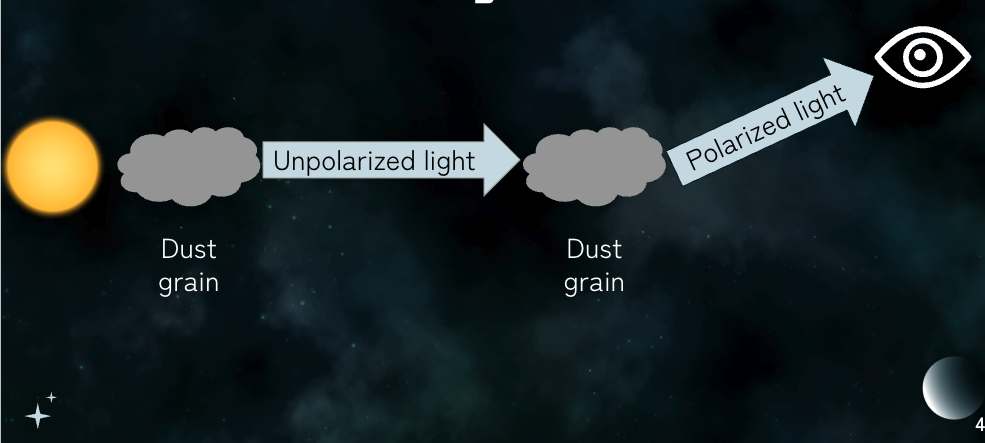
\includegraphics[width=0.8\textwidth]{../IMAGES/SLIDESHOW_SCREENSHOT/dust_self_scattering_schematic.png}
  \caption{\add{caption}}
  \label{fig: dust-self-scattering-schematic}
\end{figure*}
% ------------------------------------------------







%%%%%%%%%%%%%%%%%%%%%%%%%%%%%%%%%%%%%%%%%%%%%%%%%%
\subsubsection{Radiative Alignment}
%%%%%%%%%%%%%%%%%%%%%%%%%%%%%%%%%%%%%%%%%%%%%%%%%%




%%%%%%%%%%%%%%%%%%%%%%%%%%%%%%%%%%%%%%%%%%%%%%%%%%
\subsection{Polarization Morphologies}
%%%%%%%%%%%%%%%%%%%%%%%%%%%%%%%%%%%%%%%%%%%%%%%%%%
\note{Pattern due to polarization}



%%%%%%%%%%%%%%%%%%%%%%%%%%%%%%%%%%%%%%%%%%%%%%%%%%
\subsection{Why polarization is useful}
%%%%%%%%%%%%%%%%%%%%%%%%%%%%%%%%%%%%%%%%%%%%%%%%%%


















% ------------------------------------------------
\begin{figure*}[h]
  \centering
  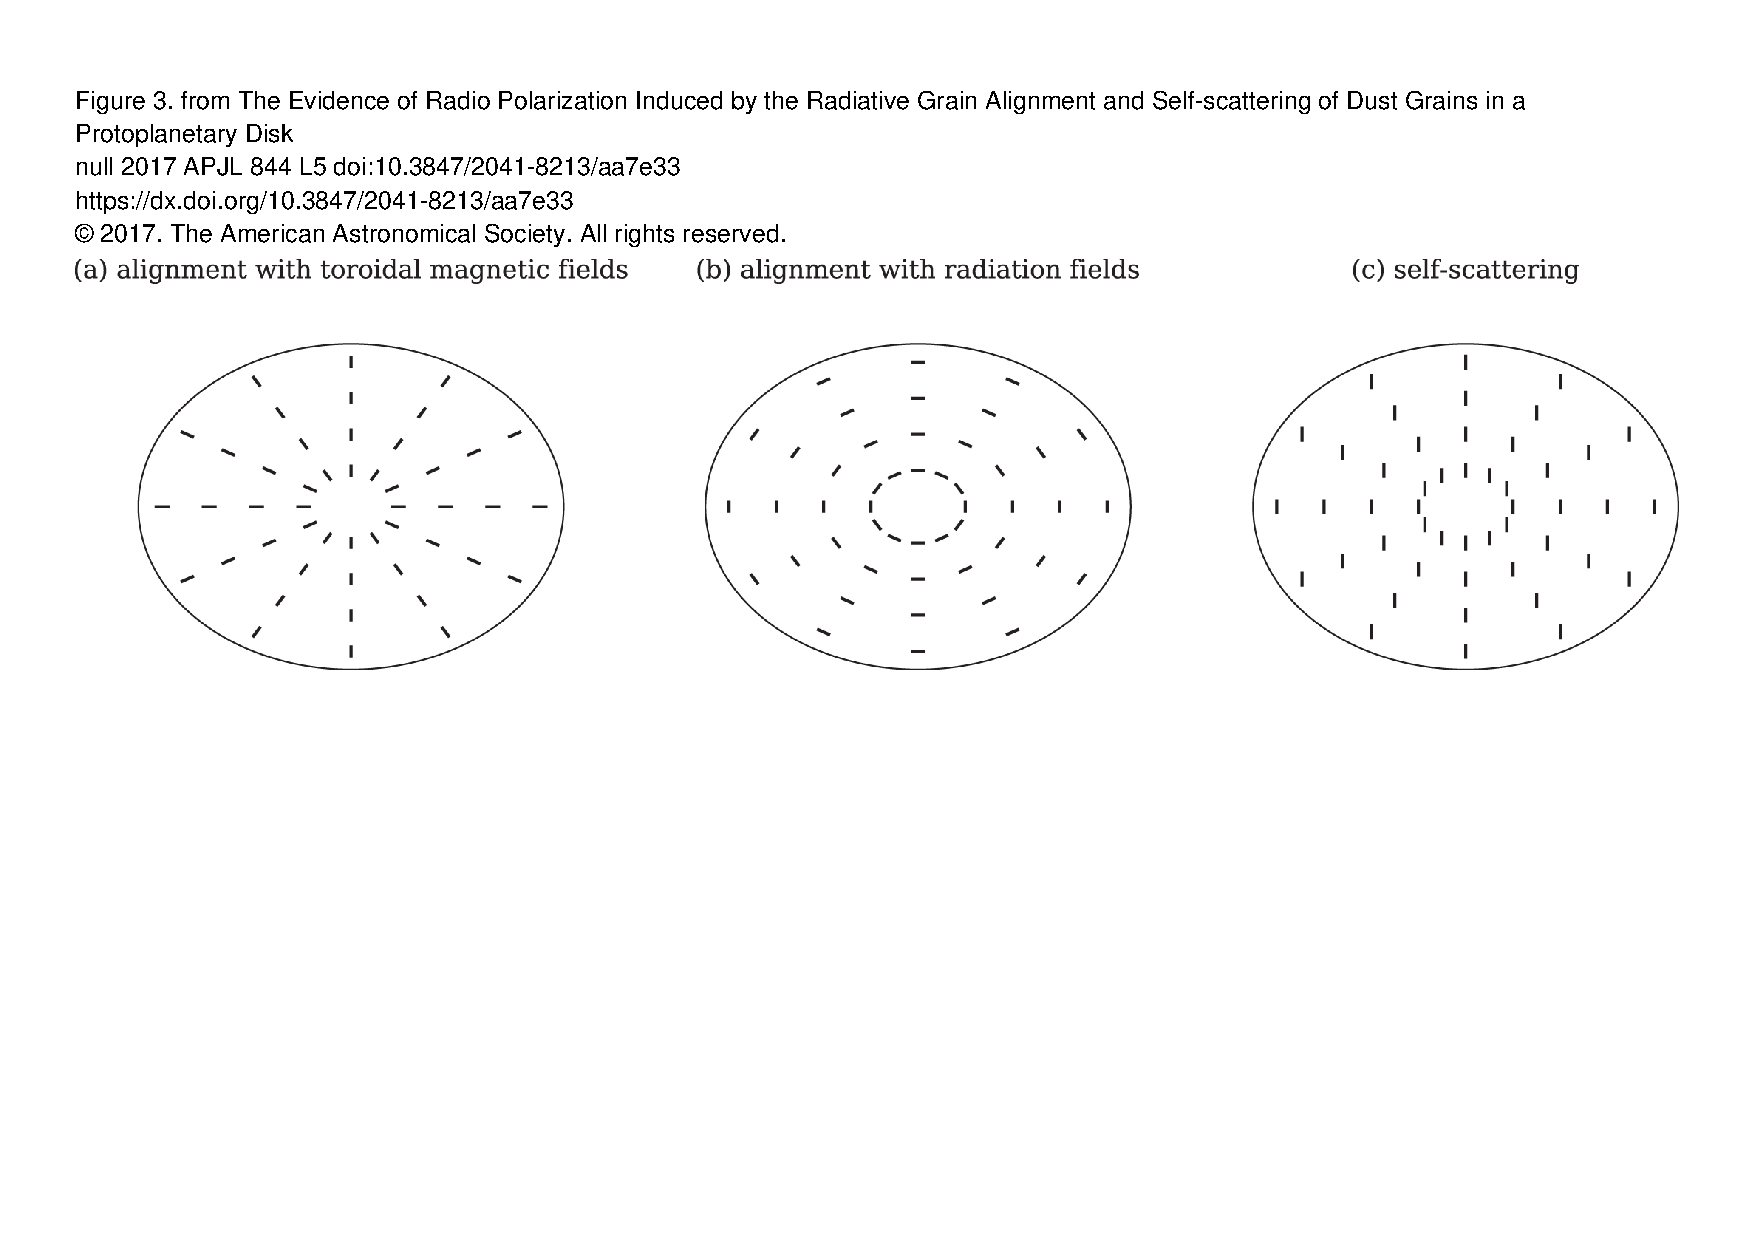
\includegraphics[width=0.8\textwidth]{../IMAGES/WRITEUP/FromPapers/Kataoka2017Figure3.pdf}
  \caption{\add{caption} \note{ask permission to use} \note{I will take off the top part and make it larger, better quality, etc}}
  \label{fig: kataoka_polarization_morphologies}
\end{figure*}
% ------------------------------------------------




